% Drawing 161-2/03-1 -- folder 161-2, batch 03, archive page 47 (PDF page 48).
% Transcription: sous les mots encerclés « Topos non cohérent », un croquis : deux ovales « $Z'$ » et « $Z''$ » qui se recouvrent, la région commune marquée « $I$ » ; au-dessus, entre les deux, « $W$ » ; au-dessous, un trait terminé par une pointe vers le bas.
% Kind: two overlapping ovals with a marked intersection, two braces labelled w and v. Method 2 (schematic redraw from the facsimile). Status: partial.
% Notes: Two ovals overlapping: Z' on the left, Z'' on the right (tilted, rising to the right), I in the common region; above them, between the two, W, with a stroke running from it down into the common region. Redrawn 2026-11-13 after the editor's answer (#148: « c'est bien mais les traits à côté de w et v (minuscules) sont des accolades »): the small letter above W at the left is a lowercase w, and the wavy stroke beside it is a brace; the mark under the ovals is a lowercase v (not an arrow head), and the short curved stroke above it, leaving the common region, is a brace. Both braces are drawn as plain brace curves, their tips towards the letters' side as far as the page shows; their exact extent is a reading. Partial: the wavy scribbles inside Z' (left of I) and inside Z'' (right of I) are still not drawn (they may be further braces or small illegible labels); the stroke from W is drawn as one curve where the page has two passes. The ringed words above (Topos non cohérent) are not drawn. Overlaid on the 400 dpi colour crop. Not checked by a reader. Disagreement: The transcription reads « au-dessous, un trait terminé par une pointe vers le bas »: by the editor (#148) the stroke is a brace and the mark under it the letter v; the lowercase w above W and its brace are not in the transcription.
% Coordinates: 1 unit = 1 mm = 1/100 of the crop width (bbox in page fractions: [0.7, 0.37, 0.97, 0.485]).
% Redrawn by Claude (claude-opus-5-5), issues #73 and #148, 2026-11-13; not checked by a human; not compiled (no TeX in the session).
% Rights: reproduces part of the work -- behind RENDER_TRANSCRIPTS, never published by itself.
\documentclass[tikz,border=3pt]{standalone}
\usepackage{amsmath,amssymb}
\usetikzlibrary{patterns,arrows.meta}
\tikzset{pencil/.style={black!45}, struck/.style={black!35}, mark/.style={circle,draw,inner sep=1.3pt}, pt/.style={circle,fill,inner sep=0.9pt}, opt/.style={circle,draw,fill=white,inner sep=1.1pt}}
\begin{document}
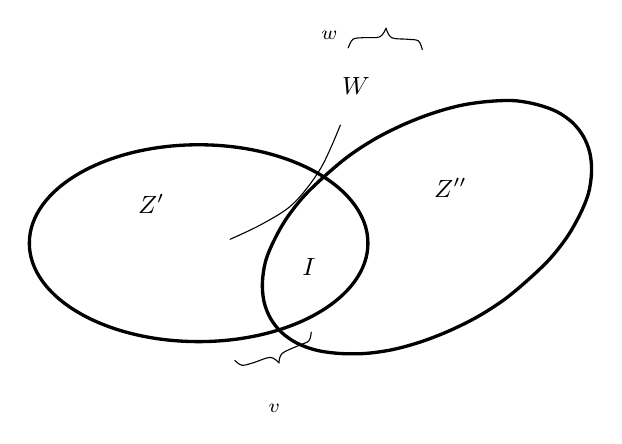
\begin{tikzpicture}[x=1mm,y=1mm,line cap=round,line join=round,font=\scriptsize]
\draw[very thick] (32,-34) ellipse[x radius=21.5, y radius=12.5];
\draw[very thick] plot[smooth cycle, tension=0.55] coordinates {(80.9,-20.5) (81.7,-22.6) (81.9,-25) (81.5,-27.7) (80.4,-30.4) (78.8,-33.2) (76.6,-36) (73.9,-38.6) (70.9,-41.1) (67.5,-43.3) (63.9,-45.1) (60.3,-46.5) (56.7,-47.5) (53.2,-48) (49.9,-48) (47,-47.6) (44.5,-46.7) (42.5,-45.3) (41.1,-43.5) (40.3,-41.4) (40.1,-39) (40.5,-36.3) (41.6,-33.6) (43.2,-30.8) (45.4,-28) (48.1,-25.4) (51.1,-22.9) (54.5,-20.7) (58.1,-18.9) (61.7,-17.5) (65.3,-16.5) (68.8,-16) (72.1,-15.9) (75,-16.4) (77.5,-17.3) (79.5,-18.7)};
\node[inner sep=1pt] at (26,-29) {\small $Z'$};
\node[inner sep=1pt] at (64,-27) {\small $Z''$};
\node[inner sep=1pt] at (46,-37) {\small $I$};
\node[inner sep=1pt] at (52,-14) {\small $W$};
\draw plot[smooth, tension=0.55] coordinates {(50,-19) (47.5,-24.5) (44,-29) (40,-31.6) (36,-33.5)};
\node[inner sep=1pt] at (48.6,-7.6) {\scriptsize $w$};
\draw plot[smooth, tension=0.55] coordinates {(51,-9.2) (51.6,-8.1) (52.9,-7.9) (55,-7.8) (55.8,-6.7)};
\draw plot[smooth, tension=0.55] coordinates {(55.8,-6.7) (56.5,-7.9) (58.5,-8.1) (59.9,-8.3) (60.4,-9.4)};
\draw plot[smooth, tension=0.55] coordinates {(46.3,-45.3) (46,-46.4) (44.7,-47) (42.6,-48) (42.2,-49.2)};
\draw plot[smooth, tension=0.55] coordinates {(42.2,-49.2) (41.1,-48.5) (38.9,-49.2) (37.5,-49.5) (36.6,-48.9)};
\node[inner sep=1pt] at (41.6,-55) {\scriptsize $v$};
\end{tikzpicture}
\end{document}
